\documentclass[../report.tex]{subfiles}
\begin{document}
\subsection{Visualisation of learned manifolds}
It is possible to observe what the encoder learnt during training if we choose a low-dimensional latent space e.g. $2D$. Following the authors, we mapped the linearly spaced grid of coordinates over the unit square through the inverse CDF of the Gaussian (our prior for the latent space is Gaussian) to obtain the value of $\mathbf{z}$. Then, we plotted the output of our decoder $p_{\mathbf{\theta}} (\mathbf{x}| \mathbf{z})$ with the estimated parameters $\mathbf{\theta}$. Figure \ref{fig:FREY} shows the results for two learned manifolds.

\begin{figure}[!htb]
\minipage{0.5\linewidth}%
\begin{center}
%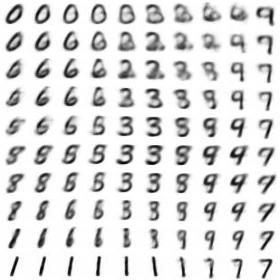
\includegraphics[width=0.6\linewidth]{../../freyFaces/MNIST.jpg}
\end{center}
\endminipage 
\minipage{0.5\linewidth}  
\begin{center}
%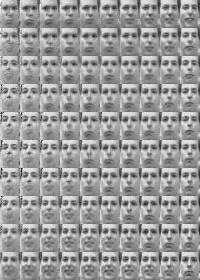
\includegraphics[width=0.5\linewidth]{../freyFaces/FREY.jpg}
\end{center}
\endminipage\hfill

  \caption[1]{Visualisations of learned data manifolds using two-dimensional latent space, trained with AEVB and Gaussian prior over the latent variable $\mathbf{z}$.}
\label{fig:FREY}
\end{figure}

In the case of the MNIST dataset, similarly to the results in the paper the central number is $3$ which corresponds to the point $(0,0)$. In the case of the second dataset, it is interesting that the first half of the manifold shows the face from left profile while the second half slowly transforms it to the right profile. Moreover, in both part of the manifold we can observe happy and grim faces which is a different representation comparing to the one obtained by the authors.

\subsection{Number of samples and a batch size}
The authors found out that the number of samples $L$ per data point can be set to $1$ as long as the mini-batch size $M$ was large enough, e.g. $M = 100$. However, they didn't provide any empirical results and we decided to run the comparison between the number of samples and a batch size in terms of optimizing the lower bound. Due to the computational requirements ($32$ models needed for evaluation), the experiment was run only with Frey Face dataset with $2000$ epochs of training. Figure \ref{fig:heatmaps} presents the results for sample size ranging from $1$ to $8$ and batches of size $20$, $60$, $100$ and $140$.
\begin{figure}[!htb]
\minipage{0.5\linewidth}%
%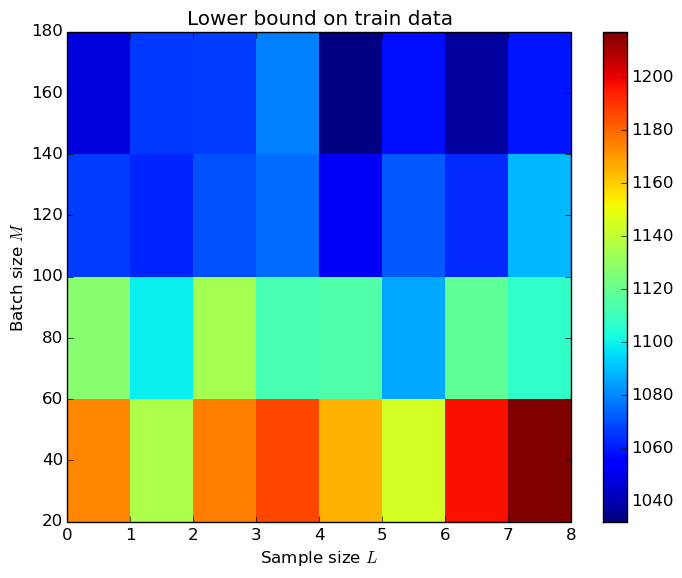
\includegraphics[width=0.7\linewidth]{../res/heatMapTraining}
\endminipage 
\minipage{0.5\linewidth}  
%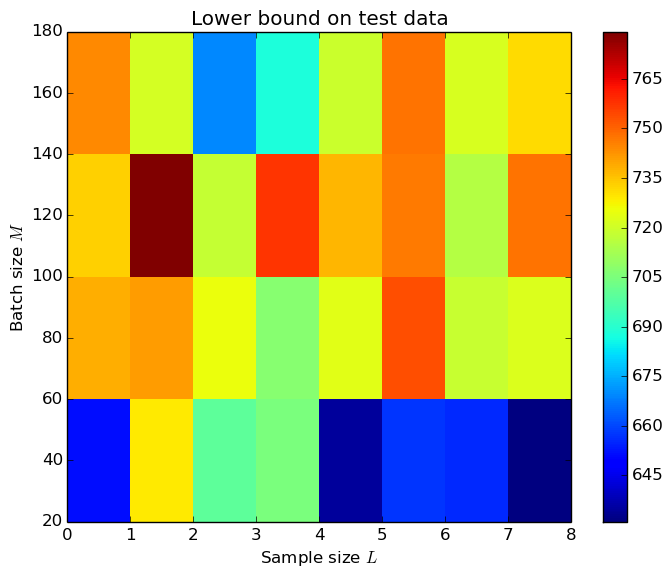
\includegraphics[width=0.7\linewidth]{../res/heatMapValid}
\endminipage\hfill
  \caption[1]{Heatmaps of lower bound for Frey Face data set.}
  \label{fig:heatmaps}
\end{figure}

The results are somewhat inconclusive and don't confirm the authors' findings. In the case of the test data, the highest score was obtained with $L=2$ and $M=100$ and the score was invariant to the sample size only with the batch size larger than $20$. In the case of training set, the highest score for lower bound was obtained with the batch of size $20$ where the sample size $L$ makes a big influence. For larger sizes of batch sample size becomes invariant in terms of the score for the lower bound. However, it is possible that the models trained with a larger batch size might need more time to converge and and further investigation is needed here.

\subsection{Increasing the depth of the encoder}
Extending the depth of the neural networks proved to be a very helpful method in increasing the power of neural architectures. The authors considered the encoder with only one hidden layer and we decided to add additional hidden layers to test how much gains can be obtained in terms of optimizing the lower bound and at the same time still obtaining robust results. The experiment was run with MNIST data set having $500$ hidden units with the size of the latent space $N_z$ set to $10$ which seems to be optimal value. 

\begin{figure}[!htb]
\centering
%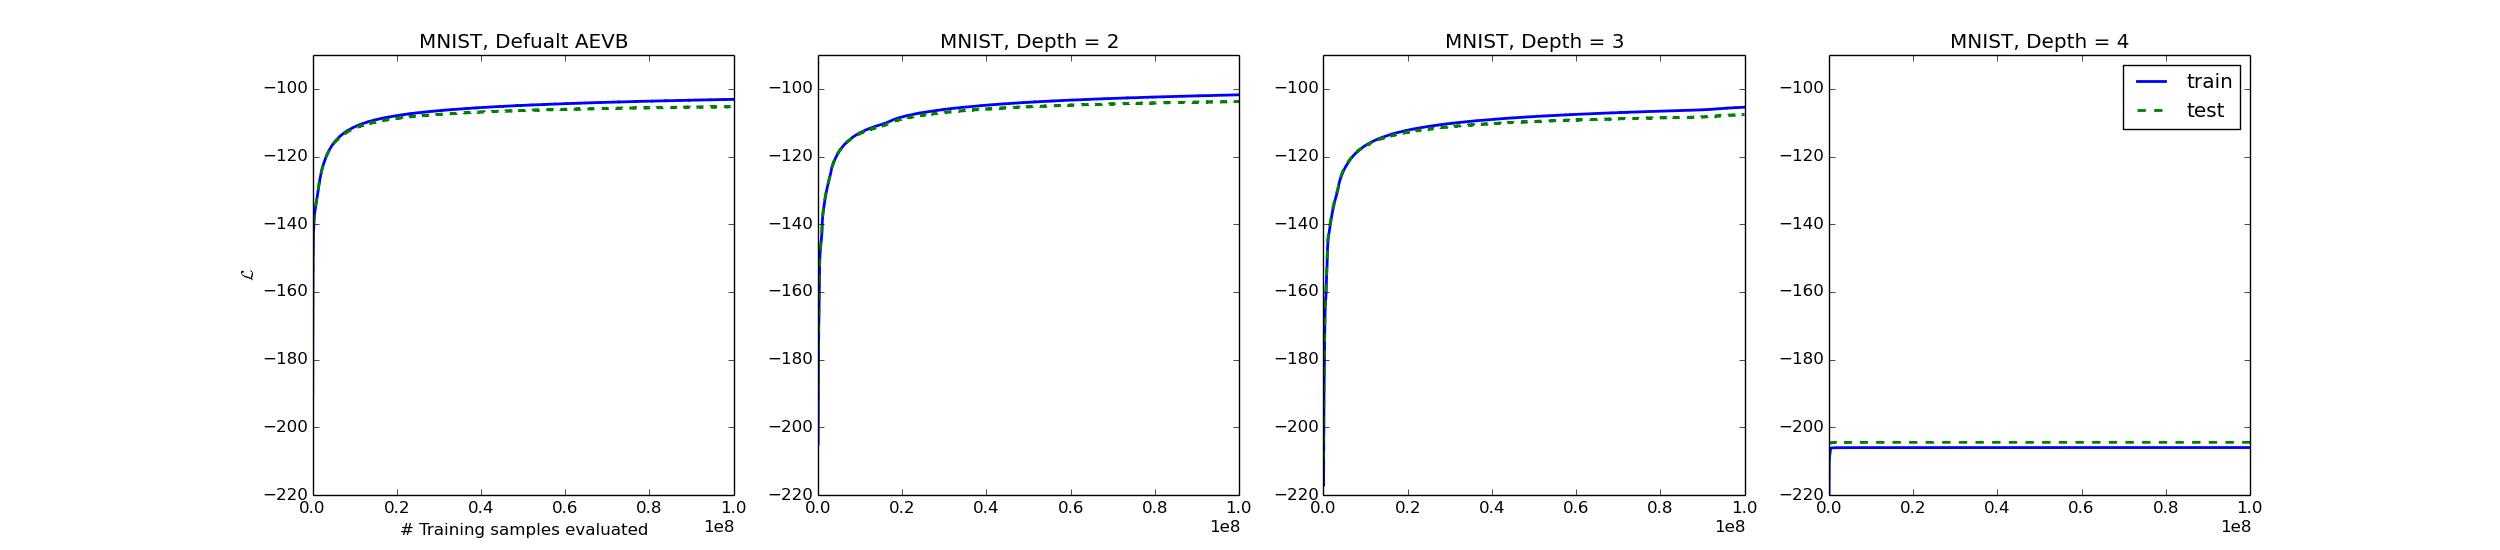
\includegraphics[width=0.8\linewidth]{../../res/mnist_depth}
%\includegraphics[width=0.8\linewidth]{../res/frey_LAvsLB}

  \caption[1]{Comparison of performance between different encoders architectures in terms of optimizing the lower bound with dimensionality of latent a space set to $10$. }
\end{figure}

Additional hidden layers didn't yield substantial increase in the performance however the encoder with two hidden layers performed slightly better than the original architecture. As it was expected, adding fourth hidden layer resulted in the inability of the network to learn.

\subsection{Noisy KL-divergence estimate}
Until now we were assuming that the $KL$-divergence term $D_{KL} (q_{\phi}(\mathbf{z} | \mathbf{x}^{(i)}) || p_{\boldsymbol{\theta}}( \mathbf{z}) ) $ can be obtained using a closed-form expression. However, in the case of the non-Gaussian distributions it is often impossible and this term also requires estimation by sampling. This is called by authors as a generic SGVB estimator $\widetilde{\mathcal{L}}^{A}(\boldsymbol{\theta}, \boldsymbol{\phi}; \mathbf{x}^{(i)})$ of the form:

$$ \widetilde{\mathcal{L}}^{A}(\boldsymbol{\theta}, \boldsymbol{\phi}; \mathbf{x}^{(i)}) = \frac{1}{L} \sum_{l=1}^L \left( \log p_{\boldsymbol{\theta}}(\mathbf{x}^{(i)}, \mathbf{z}^{(i,l)}) - \log q_{\phi}(\mathbf{z}^{(i,l)} | \mathbf{x}^{(i)}) \right).$$

Naturally, this form in general will have greater variance than the previous estimator. We decided that it will be informative to compare the performance of both estimators using only one sample i.e. $L=1$ -- this will allow us to observe how much more robust is the first estimator. Figure \ref{fig:mnist_LAvsLB} shows the results for the MNIST data set where lower bound for $\widetilde{\mathcal{L}}^{B}$ was taken from the section $?$.

\begin{figure}[!htb]
\centering
%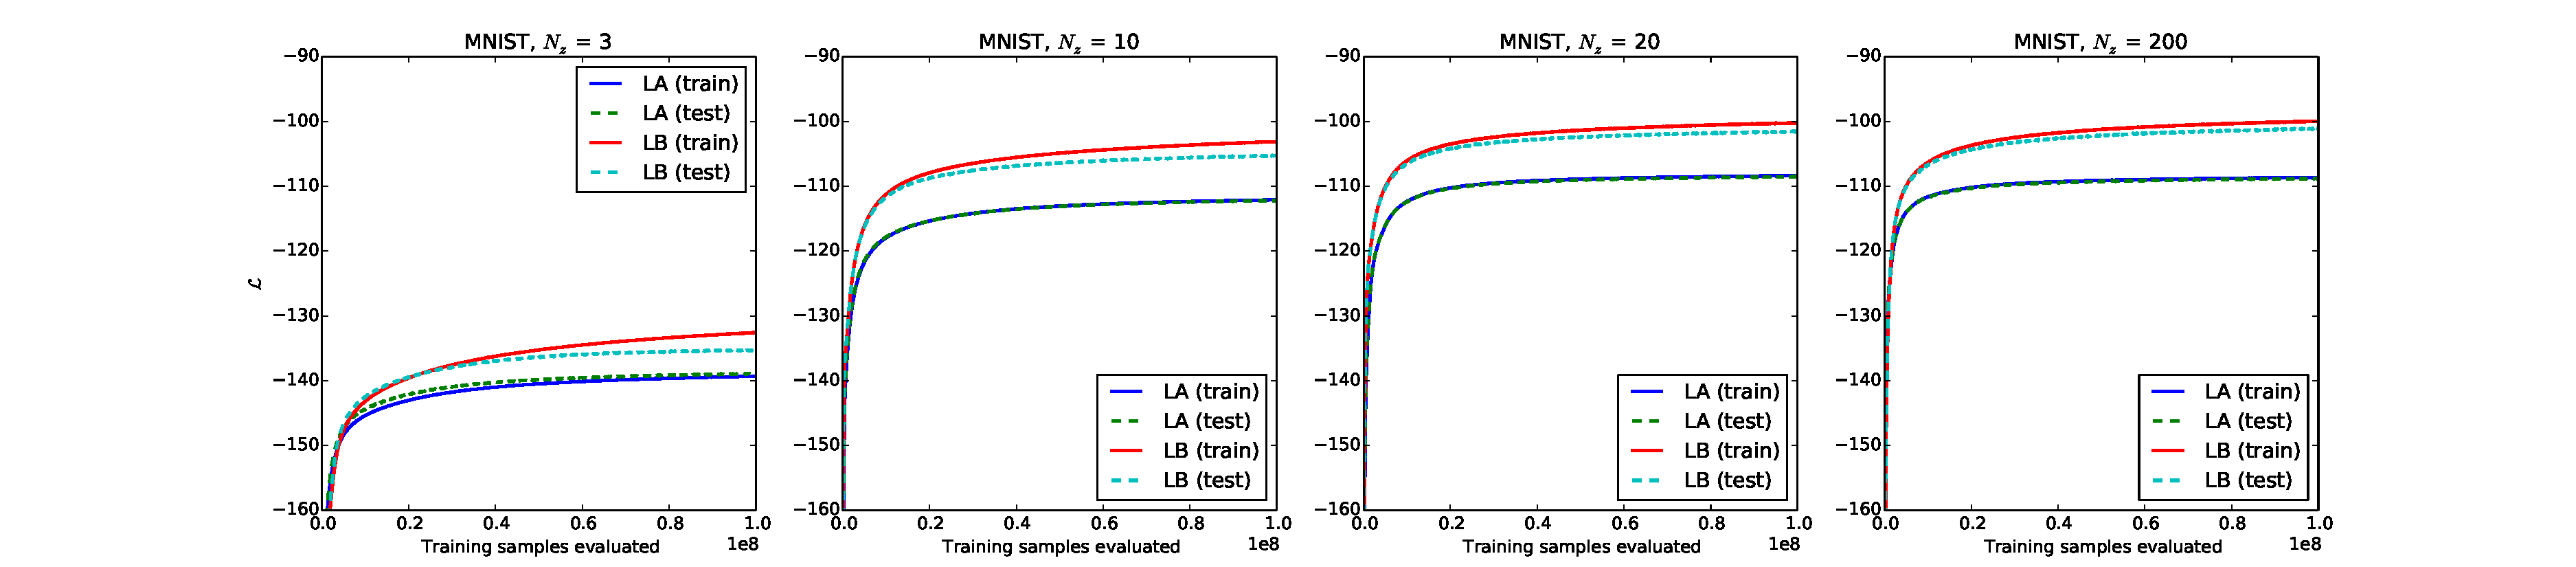
\includegraphics[width=0.8\linewidth]{../../res/mnist_LAvsLB}
%\includegraphics[width=0.8\linewidth]{../res/frey_LAvsLB}

  \caption[1]{Comparison of two SGVB estimators in terms of optimizing the lower bound for different dimensionality of latent space ($N_z$). }
  \label{fig:mnist_LAvsLB}
\end{figure}

As we can see, in each case the performance of the $\widetilde{\mathcal{L}}^{B}$ estimator is substantially better. Moreover, this shows that the generic estimator might be used if we increase the sample size $L$ to reduce the variance of the estimator. However, this needs to be examined empirically. Moreover, this comes with higher computational costs.

\subsection{Activation functions}
The paper considered only $\text{tanh}$ as an activation function in the case of hidden layers. That is why, we tested also sigmoid and ReLu activation functions for different size of latent variable space $N_z$ to compare differences in terms of optimising lower bound and computational efficiency. Figure \ref{fig:mnist_activation} shows results for three such set-ups with the size of the latent space  $N_z$ set to $10$ for MNIST data set.

\begin{figure}[!htb]
\centering
%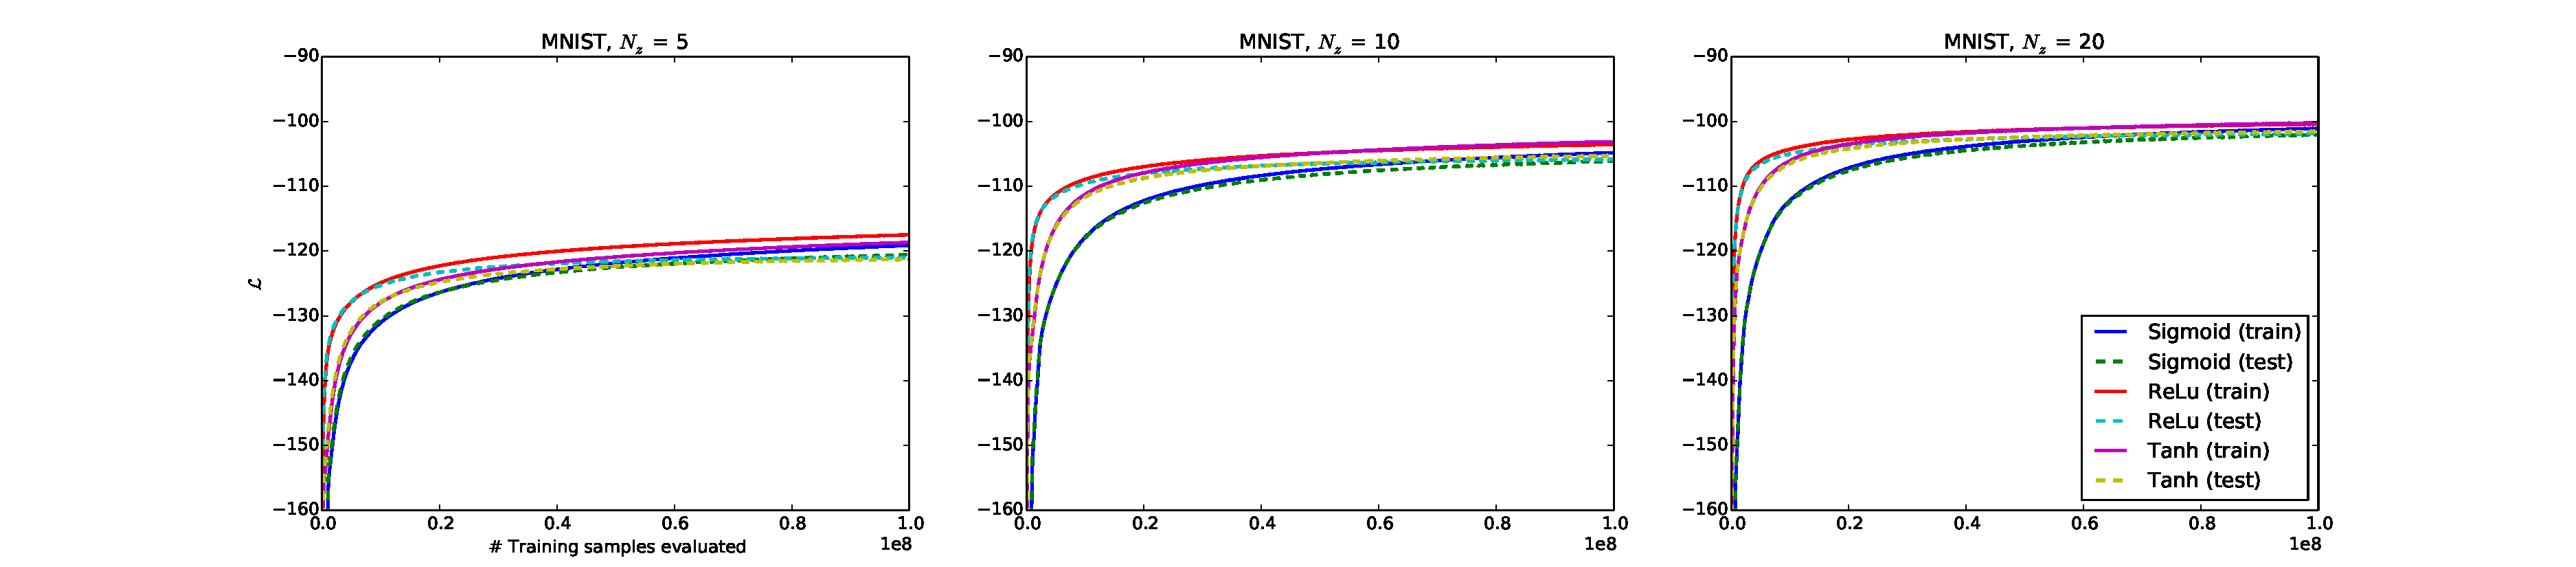
\includegraphics[width=0.8\linewidth]{../../res/mnist_activations}
%\includegraphics[width=0.8\linewidth]{../res/frey_LAvsLB}
  \caption[1]{Comparison of different activation functions in terms of optimizing the lower bound. }
\label{fig:mnist_activation}
\end{figure}

Although, as it was expected, ReLu function learns the fastest, there is no substantial gains over tanh function. In each case, the sigmoid function learns the slowest and obtains the lowest score for the bound and at the same time the training time took about $20\%$ more time than in the case of the two other functions.

\end{document}
